\documentclass{standalone}
\usepackage{tikz}
\usetikzlibrary{matrix,arrows,positioning}

\begin{document}
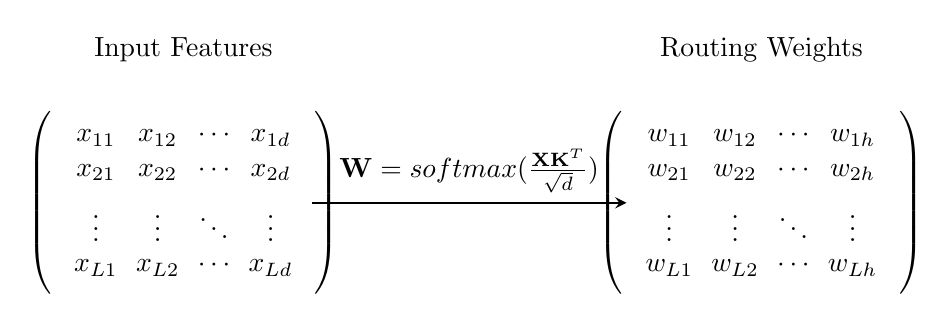
\begin{tikzpicture}[
    node distance=2cm,
    box/.style={rectangle,draw,rounded corners,fill=blue!10,minimum width=2cm,minimum height=1cm},
    arrow/.style={->,>=stealth,thick}
]

% Input matrix
\matrix (input) [matrix of math nodes, left delimiter=(, right delimiter=)]
{
x_{11} & x_{12} & \cdots & x_{1d} \\
x_{21} & x_{22} & \cdots & x_{2d} \\
\vdots & \vdots & \ddots & \vdots \\
x_{L1} & x_{L2} & \cdots & x_{Ld} \\
};

% Routing weights
\matrix (weights) [matrix of math nodes, right=4cm of input, left delimiter=(, right delimiter=)]
{
w_{11} & w_{12} & \cdots & w_{1h} \\
w_{21} & w_{22} & \cdots & w_{2h} \\
\vdots & \vdots & \ddots & \vdots \\
w_{L1} & w_{L2} & \cdots & w_{Lh} \\
};

% Labels
\node[above=0.5cm of input] {Input Features};
\node[above=0.5cm of weights] {Routing Weights};

% Routing operation
\draw[arrow] (input) -- node[above] {$\mathbf{W} = \text{softmax}(\frac{\mathbf{X}\mathbf{K}^T}{\sqrt{d}})$} (weights);

\end{tikzpicture}
\end{document}
